\documentclass[12pt,twoside]{article}
\usepackage[utf8]{inputenc}
%\usepackage{CClicenses}
\usepackage{jeffe}
\usepackage[hmargin=1in,vmargin=1in]{geometry}

%% Used for PgfPlots example, shown in the "Figures" section below.
\usepackage{pgfplots}
\pgfplotsset{compat=1.14}

\usepackage{cite}
\usepackage{cleveref}
\usepackage{xspace}
\usepackage{enumitem}
\usepackage{amsopn}
\usepackage{verbatim}
\usepackage{mathtools}

%------------------------------------------
% line numbers
%------------------------------------------
\usepackage[mathlines]{lineno}
%pagewise
%\linenumbers
\renewcommand\linenumberfont{\normalfont\tiny\sffamily\color{Gray}}
\setlength\linenumbersep{2em}

\DeclareMathOperator{\Range}{Range}
\DeclareMathOperator{\Lg}{lg}
\DeclareMathOperator{\Argmin}{argmin}
\DeclareMathOperator{\Argmax}{argmax}
\DeclareMathOperator{\Poly}{\poly}
\DeclareMathOperator{\Polylog}{\polylog}
\DeclareMathOperator{\Lin}{Lin}
\DeclareMathOperator{\dist}{dist}
\DeclareMathOperator{\probability}{\mathbb{P}}
\DeclareMathOperator{\cat}{cat}
\DeclareMathOperator{\Dim}{dim}

\def\distG{\dist_{G^*}}
\def\eps{\varepsilon}
\def\cost{\textsc{Cost}}
\def\spread{\textsc{Sp}}
\def\dartof#1{\vec{#1}}
\def\dartsof#1{\dartof{#1}}
\def\event{e}
\def\R{\mathbb{R}}

%% ------------------------------------------------------------------
%% End of macros for in-document examples.
%% ------------------------------------------------------------------

\newtheorem{lemma}{Lemma}[section]
\newtheorem{theorem}[lemma]{Theorem}
\newtheorem{corollary}[lemma]{Corollary}
\newtheorem{observation}[lemma]{Observation}
\newtheorem{claim}[lemma]{Claim}
\newtheorem{definition}[lemma]{Definition}
\newtheorem{example}[lemma]{Example}

% \theoremstyle{plain}

\begin{document}
\title{A Survey on Topology in Motion Planning}

\author{
Dongpeng Liu %
and Jiashuai Lu%
}

%\DRAFT

\maketitle

%
\begin{abstract}
  Motion Planning is a computational problem that, given an object and a set of obstacles, how can we move the object from a source point to a destination point without colliding with any obstacle.
  The problem has many robotic applications, such as autonomy, automation, artificial intelligence, etc. It is studied by both computational geometry community and robotics community.
  In this paper we discuss several applications of topology on motion planning.
  We study in detail the configuration space of motion planning problem, and some numerical homotopy invariant of any path-connected topological space \(X\). We discuss how those invariant measure the ``complexity of the problem of navigation in \(X\)'' and determines the structure of motion planning algorithms in \(X\).
  We introduce the useful properties of topological map for motion planning and how to build a ``good'' topological map. The interest of having multiple homotopically distinct paths into consideration also suggest us to study the approximate path similarity metrics.
\end{abstract}

\setcounter{page}{0}
%\thispagestyle{empty}

\section{Introduction}\label{sec:intro}
%%% Local Variables:
%%% mode: latex
%%% TeX-master: "report"
%%% End:

At every moment, we are making plans of our actions for the very next instant.
Planning is involved in everywhere in our daily life, for example, which route we use to get to work, how to make a drone able to get back safely by itself.
Motion planning, is a problem that given a start position \(s\) of a object \(X\) and a goal position \(t\), possibly with a set of obstacles, computes a path that moves \(X\) from \(s\) to \(t\) without colliding with any obstacle.
It is also know as the piano mover's problem.
Imagine that we are given a computer-aided design (CAD) model of a house and a piano, and the goal is determine a way to move the piano from one room to another in the house without hitting anything~\cite{lavalle2006planning}.
This problem has many applications in robotics, computational geometry, computer games, etc. Especitally in the progress of autonomous robotics, it makes a critial role in the problem of enable the robotics to make decision for their own actions based on different cases~\cite{eric98}.

While there are multiple versions of this problem according to how the obstacle information is given, researchers usually focus on the most simple version that all description of obstacles are given and fixed through the planning.
The problem in this setting is often referred as the basic motion planning problem, and it is usually solved by first building a graph to model the geometric structure of the environment and then finding a connected component that contains both the start and target positions. There are three common approaches to solve this basic setting problem: the roadmap approach, the cell decomposition approach, and the potential field approach~\cite{eric98}. The first two of them are both using the concept of \textit{configuration space}, \textit{free space} and the goal is finding a \textit{free path} where the configuration space is a transformation from the realistic space of the robot of certain shape and size into a space that the robot is shrinked to a point.


\section{Topological Complexity of a Topological Space}\label{sec:complexity}
%%% Local Variables:
%%% mode: latex
%%% TeX-master: "report"
%%% End:
In this section, we first introduce a formal definition of the motion planning problem. Then we will give the topological representation of the problem. After that, we are able to start discussing about a homotopy invariant of a path-connected topological space, which is proposed by Farber in 2003~\cite{DBLP:journals/dcg/Farber03}.

\subsection{Configuration Spaces of Motion Planning}
The word \textit{robot} was first invented by the Czech writer Karel\u{a}pek in his play R.U.R. (Rossum's Universal Robots)~\cite{zunt2002did}. But the concept of automata, can be found in many ancient mythologies. Autonomous robots, which should be able to complete many tasks without any human's control or assistance, is an essential objective of modern robotics research.

In the motion planning problem, we use \textit{configuration} to describe the object's position and possible direction(all geometric characteristics of the object).
The \textit{configuration space} is often referred to all possible configurations(states).
Typically, every configuration \(A\) consists of a finite set of real numbers, and we can see the configuration space \(X\) as a subset of the Euclidean space of which the dimension is the number of values we used to encode one state of the object.
In this setting, every point in this subset represents a state of the object.
Then we can naturally relate Topology and motion planning through the configuration space \(X\).
Given the configuration space \(X\) of a motion planning system, we may solve the problem by only looking at \(X\)'s topology properties, possibly with some necessary geometric features.

\begin{example}[Piano movers' problem~\cite{schwartz1983piano,DBLP:journals/dcg/Farber03}]
  We look at a simple version of the piano movers' problem here.
  As Figure~\ref{fig:piano} shows, the black piano shape can only move horizontally and the rectangles are obstacles.
  Let the four piano shapes be four different states of the piano.
  The problem is how to move the piano from one state to another one without colliding any obstacle.
  \begin{figure}
    \begin{center}
      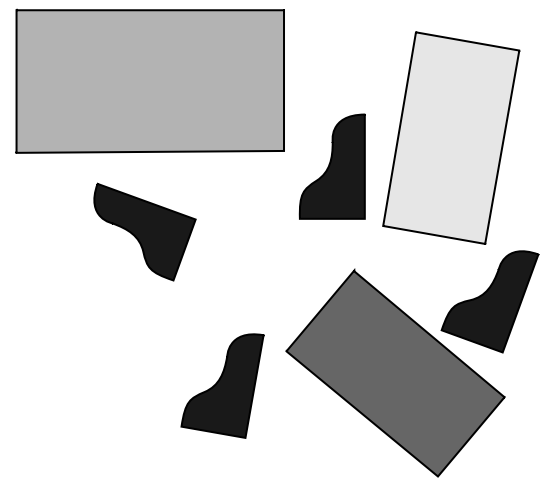
\includegraphics[width=0.5\textwidth]{fig-piano}
    \end{center}
    \caption{An example of piano mover's problem}
    \label{fig:piano}
  \end{figure}
\end{example}
In this case, every unique state of the piano can be described by three variables, two for the coordinates of the center of the piano and another one for denoting the direction.
Therefore, the configuration space of it is a subset set of \(\R^3\).

Schwartz and Sharir also give an algebraic formulation for the general version of ``Piano'' mover's problem.
In this setting, we are considering collision-free states of some hinged object \(B\), where \(B\) can be decomposed to a finite number of rigid compact subparts \(B_1,B_2,\dots,\).
Every rigit subpart is bounded by a number of algebraic surfaces.
Any two subparts \(B_1, B_2\) can be connected together by any one of following ways:
\begin{enumerate}[label=\arabic*)]
\item \(B_1\) and \(B_2\) are partially overlapping such that \(B_1\) and \(B_2\) are combined by a unique point in the overlapping part.
\item \(B_1\) and \(B_2\) are connected by a hinge between two points \(a_1, a_2\) where \(a_1\in B_1, a_2\in B_2\). In this case, \(B_2\) can revolve around some axis \(X\) fixed in the frame of \(B_1\).
\item \(B_2\) can slide and rotate along some axis \(X\) fixed in the frame of \(B_1\).
\end{enumerate}

To formulate the problem algebraically, they first describe a superspace of the set of all valid states of the hinged object \(B\).
The rotation group is a smooth \(3\)-dimensional algebraic submanifold of the \(9\)-dimensional Euclidean space of \(3\times 3\) real matrices.
Recall that an algebraic manifold is a smooth algebraic variety.
If \(B\) itself is minimal, i.e., \(B\) is a rigit compact subpart. Then its state can be represented by an Euclidean motion \(T\) from some base state to the given state.
The transformation \(Ts=Rs+s_0\) is defined by a pair \((s_0, R)\) where \(s_0\) is a point in \(\R^3\) and \(R\) is a rotation matrix described above.
So the transformation can be seen as a point in a smooth \(6\)-dimensional algebraic submanifold of \(\R^{12}\).

Otherwise, \(B\) consists of multiple parts throught different ways listed earlier. One could find that in all cases, the overall states of all parts can be represented as a point in a smooth algebraic manifold in a Euclidean space of some dimension. For more details including a general path-finding algorithm runs in time exponential in the number of degrees of freedom of the object, we refer to ~\cite{schwartz1983piano}.

\begin{example}[The robot arm~\cite{latombe2012robot,DBLP:journals/dcg/Farber03}]
  In 1991, Latombe described a general robot arm problem. An arm is constituted by connecting a couple of bars through revolving joins as Figure~\ref{fig:arm} shows.
  \begin{figure}
    \begin{center}
      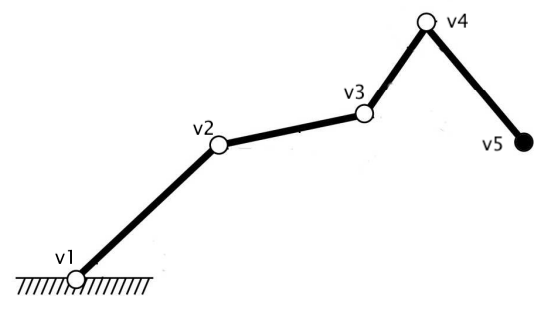
\includegraphics[width=0.5\textwidth]{fig-arm}
    \end{center}
    \caption{An example of the robot arm problem}
    \label{fig:arm}
  \end{figure}
\end{example}
Assume bars of the arm can have self-intersections. If the arm is in 2-dimensional plane, fix any \(v_i\), the configuration space of \(v_{i+1}\) is \(S^1\). Therefore, the whole configuration space \(X\) is:
\[\underbrace{S^1\times S^1\times\dots\times S^1}_{\text{\# of bars}}\]
Similarly, in 3-dimensional space, the configuration space \(X\) is:
\[\underbrace{S^2\times S^2\times\dots\times S^2}_{\text{\# of bars}}\]

\subsubsection{General Configuration Spaces}
Let \(A\) be a topological space and \(Q_m=\{q_i|1\le i\le m, q_i\in A\}\) be a subset of points in \(A\) representing obstacles.
Let \(B=A-Q_m\) and let \(X=F(A,m,n)\) denote some subset of \(\underbrace{B\times B\times\dots\times B}_{n}\) such that
for every element \(E=(e_1,e_2,\dots,e_n)\) in \(X\), every \(e_i\) of \(E\) has a unique value in \(B\).
Then \(F(A,m,n)\) is the collision-free configuration space of a system of \(n\) points moving in space \(A\).
% Fadell and Neuwirth gave the configuration spaces \(F(\R^m,n)\) which is a special case of \(A=\R^m\) is \(m\)-dimensional Euclidean space (or an arbitrary manifold)~\cite{fadell1962configuration}.
When \(G\) is a connected graph, the configuration spaces \(F(G,m,n)\) are studied usually in robotics.

\subsubsection{Topology of Configuration Spaces of Polygonal Linkages}
In general, a linkage is a graph with fixed edge lengths. Figure~\ref{fig:linkage1} shows some linkages of various types. Let \(L\) be any graph with given edge lengths. A \textit{configuration} of \(L\) is a geometric realization of \(L\) in Euclidean space.
A \textit{reconfiguration} is a continuous sequence of such configurations (see ~\ref{fig:reconfig} for example).
The configuration space \(X\) consists of all configurations and paths corresponding to reconfigurations~\cite{connelly2004geometry}.
\begin{figure}
  \centering
  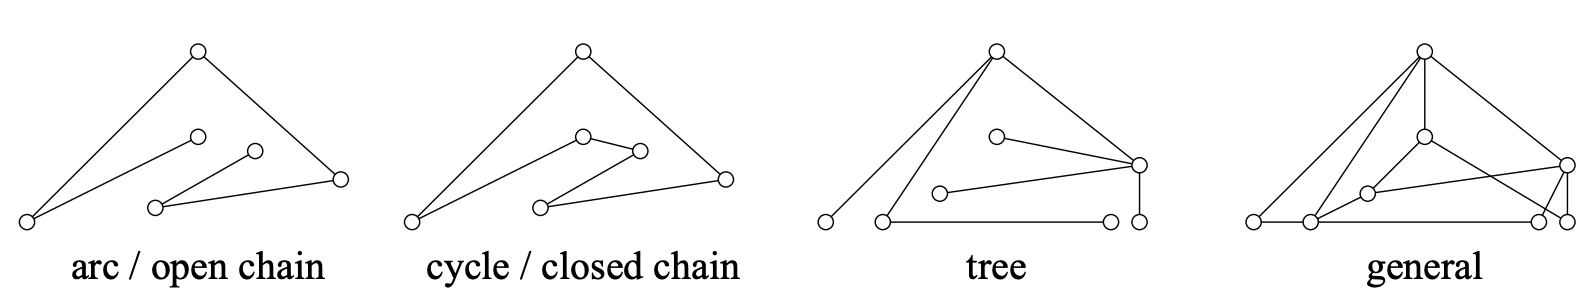
\includegraphics[width=0.9\textwidth]{fig-linkage1}
  \caption{Examples of different type linkages~\cite{connelly2004geometry}}
  \label{fig:linkage1}
\end{figure}

\begin{figure}
  \centering
  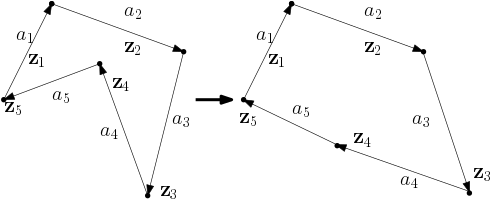
\includegraphics[width=0.9\textwidth]{fig-reconfig}
  \caption{An example of reconfiguration of a linkage}
  \label{fig:reconfig}
\end{figure}

There are a lot of results in studies on algebraic topological invariants of this configuration space.
Here we study the topology of the configuration space of linkage of cycle, which are important manifolds representing shapes of closed polygonal chains.

Let \(\mathbf{a}\) be any vector in \(\R^m_{+}\), where \(\mathbf{a}=(a_1,a_2,\dots,a_m)\) consists of \(m\) positive real numbers. Then we define the variety \(M(a)\) as:
\[M(\mathbf{a})=\{(z_1,z_2,\dots,z_m);z_i\in S^2, \sum^m_{i=1}a_iz_i=0\}/SO^3\]

Here \(SO^3\) performs as diagonal of the product \(\underbrace{S^2\times \dots \times S^2}_{n}\), and \(M(\mathbf{a})\) describes the variety of all closed polygonal shapes in \(3\)-dimensional space where the side lengths are defined by \(\mathbf{a}\). As an example, Figure~\ref{fig:reconfig} shows two different shapes with different coefficients \((z_1,z_2,\dots,z_m)\) as the orientations of edges with same edge lengths.

Given the above definition of the variety of polygonal linkage, intuitively, we have the following lemma from the triangle inequality.
\begin{lemma}\label{lm:nonempty}
  Let \(||\mathbf{a}||=\sum^m_{i=1}a_i\). \(M(\mathbf{a})\) is nonempty if and only if \(a_i<||\mathbf{a}||\) for \(1\le i\le m\).
\end{lemma}

We say a vector \(\mathbf{a}\in \R^m_+\) is \textit{generic} if \(M(\mathbf{a})\) does not include an element \(\mathbf{z}=(z_1,z_2,\dots,z_m)\) such that \(z_i=\pm{1}\) for all \(i\).

\begin{lemma}
If \(\mathbf{a}\) is generic, then \(M(a)\) is a closed smooth manifold of dimension \(2(m-3)\)~\cite{DBLP:journals/dcg/Farber03}.
\end{lemma}

To learn the relation between the variety of \(\mathbf{a}\) and \(\mathbf{a}\), we need first define the \textit{short} subset of \(\{1,2,\dots,m\}\).
We say a subset \(V\subseteq \{1,2,\dots,m\}\) if such that \(\sum_{i\in V}a_i\le \sum_{j\notin V}a_j\).
From Lemma~\ref{lm:nonempty} we know every subset \(V\) contains only a singleton is short subset.
Let \(S(\mathbf{a})\) denote all short subsets corresponding to \(\mathbf{a}\). Note that \(S(\mathbf{a})\) is partially ordered set which is determined by its maximal elements.

Hausmann and Knutson proved the following lemma of a property of the variety and short subsets in 1998.
\begin{lemma}
If two vectors \(\mathbf{a}, \mathbf{a}'\in \R^m_+\) are generic, and there is an isomorphism between \(S(\mathbf{a})\) and \(S(\mathbf{a}')\), then \(M(\mathbf{a}\) and \(M(\mathbf{a}'\) are diffeomorphic.
\end{lemma}

Recall that two smooth manifolds \(X, Y\) are diffeomorphic if there is a bijective and differentiable map \(f:X\to Y\) and \(f^{-1}\) is differentiable.

There are also some universality theorems focusing on the topological properties of the configuration spaces of linkages.

\begin{theorem}[Jordan and Steiner '98~\cite{jordan1999configuration}]
  Any compact real algebraic variety \(V\subset \R^n\) is homeomorphic to the union of components of the configuration space of a mechanical linkage.
\end{theorem}

\begin{theorem}[Kapovich and Millson '02~\cite{kapovich2002universality}]
  For any smooth compact manifold \(X\), there is a linkage \(L\) of which the moduli space is diffeomorphic to a disjoint union of a number of copies of \(X\).
\end{theorem}
Recall that the moduli space is the solutions of a geometric problem.

\subsection{Navigational Complexity of the Motion Planning Problem}
Farber explored the topological properties of the robot motion planning problem and showed that there is a homotopy invairant quantity of configuration spaces \(X\) called the \textit{navigational complexity} \(TC(X)\)~\cite{farber2003topological,farber2004instabilities}.
This invariant  explains how knowing the cohomology algebra of
configuration space of a robot one may predict instabilities of its behavior.

Let \(X\) denote the configuration space of a mechanical system \(S\)
Then we can use a continious path \(\gamma:[0,1]\to X\) to represent a sequence of continuous motions of \(S\) where \(\gamma(0),\gamma(1)\) are the initial and final states of the system, respectively.

If \(X\) is path-connected, it is easy to see that one may move the system between any two states.
Let \(PX\) denote the space of all these continuous paths.
Let \(\pi:PX\to X\times X\) be the map from path to initial-final states configuration.
Then \(\pi\) is a Serre fibration.

On the other hand, a motion planning algorithm is a function \(s:X\times X\to PX\), and \(s\) is a section of \(\pi\).

Now we are going to learn the continuity of motion planning algorithms.
We say a motion planning algorithm \(s\) is continuous if solutions \(s(A,B)\) for all \(A,B\in X\times X\) continously depend on initial-final states \(A\) and \(B\).

\begin{lemma}[Farber '03~\cite{farber2003topological}]
There exists a continuous motion planning algorithm for a configuration space \(X\) if and only if \(X\) is contractible.
\end{lemma}
In practice, most of planning problems involves noncontractible configuration spaces.
So we want to learn more about the \(discontinuities\).
Farber proposed an invariant \(\mathbf{TC}(X)\) to measure the complexity the planning problem in space \(X\).
Besides this, they also described four different ways in which \(\mathbf{TC}(X)\) affects the structure of motion planning algorithms for \(X\).
To describe those, we first use four distinct notions of navigational complexity of topological spaces: \(\mathbf{TC}_j(X), j=1,2,3,4\).

A topological space \(X\) is called an \textit{Euclidean Neighbourhood Retract} if it can be embedded into an Euclidean space \(\R^k\) such that for some open neighbourhood \(U, X\subset U\subset \R^k\), there exists a retraction \(r:U\to X,r|_X=\mathbf{1}_X\)~\cite{farber2004instabilities}.
\begin{definition}\label{def:tame}
  A motion planning algorithm \(s:X\times X\to PX\) is called \emph{tame} if \(X\times X=\Union_{1\le i\le k} P_i\) for some finited number \(k\) such that
  \begin{enumerate}[label=\arabic*)]
  \item \(s|_{P_i}:P_i\to PX, 1\le i\le k\) is continuous.
  \item All \(P_i\) are disjoint with each other.
  \item Every \(P_i\) is an ENR
  \end{enumerate}
\end{definition}

In practice, all motion planning algorithms are tame and the function \(s\) restrict to any \(P_i\) is usually real algebraic and continuous.

\begin{definition}
  The topological complexity of a tame motion planning algorithm \(s\) is the minimal number of domains of continuity \(k\) in a representation of \(s\) in definition~\ref{def:tame}~\cite{farber2006topology}.
\end{definition}

\begin{definition}
  The topological complexity \(\mathbf{TC}_1(X)\) of a path-connected topological space \(X\) is the minimal topological complexity of motion planning algorithms of \(X\)~\cite{farber2006topology}.
\end{definition}

Observe that \(\mathbf{TC}_1(X)=1\) if and only if \(X\) is a contractible Euclidean Neighbourhood Retract.
If there is no tame motion planning algorithm for \(X\), \(\mathbf{TC}_1(X)=\infty\).

Before we introduce the second notion of the topological complexity of topological spaces, we need first introduce the Schwarz genus.
Let \(\pi: X\to B\) be a fibration. Let \(k\) be a number such that there is an open cover of the base \(B=\Union_{1\le i\le k} S_i\) of which for each set \(S_i\), there is a continuous section \(s_i:U_i\to X\) of \(\pi\).
The Schwarz genus is defined as the minimum \(k\) satisfies this condition by Schwarz in 1958~\cite{schwarz1962genus}.

\begin{definition}
  Let \(X\) be any path-connected topological space. The topological complexity \(\mathbf{TC}_2(X)\) is the Schwarz genus of the fibration~\cite{farber2006topology}
  \[\pi:PX\to X\times X\]
\end{definition}

Let \(\cat(X)\) denote the Lusternik-Schnirelmann category of \(X\)~\cite{cornea2003lusternik}, then
\[\cat(X)\le \mathbf{TC}_2(X)\le \cat(X\times X)\]

The third notion of the topological complexity relates to the \emph{order of instability} of motion planning algorithms introduced by \(Farber\) in 2004. For more details, see ~\cite{farber2004instabilities}.
The order of instability is a fundamental feature of a motion planning algorithm.
Formally, it is defined as the maximum value \(r\le k\) such that for any \(\epsilon>0\) we can find \(r\) pairs of initial-final configurations \((A_1,B_1),(A_2,B_2),\dots,(A_r,B_r)\) in where the distance between any two pairs is less than \(\epsilon\) and every pair belongs to a unique set \(P_i\) as defined in definition~\ref{def:tame}.

\begin{definition}
  The topological complexity \(\mathbf{TC}_3(X)\) is the minimum order of instabilities of all tame motion planning algorithms in \(X\)~\cite{farber2006topology}.
\end{definition}

Before describing how \(\mathbf{TC}_4(X)\) is defined, we first introduce the complexity of random motion planning algorithms~\cite{farber2004collision}.

Let \(X\) be any path-connected topological space and \(PX\) be the space of all continuous paths.
\begin{definition}
  For any \(A,B\in X\), let \(\gamma_1,\gamma_2,\dots,\gamma_n\in PX\) be an order sequence of continuous paths such that \(\gamma_i(0)=A,\gamma_i(1)=B\) for any \(i\), and \(p_1,p_2,\dots,p_n\in [0,1]\) is a sequence of probabilities summing to \(1\). Then a random n-valued path \(\sigma\) from \(A\) to \(B\) is defined as:
  \[\sigma=p_1\gamma_1+\dots+p_n\gamma_n\]
\end{definition}

Let \(P_nX\) denote the set of all \(n\)-valued random paths in \(X\).
Let \(\pi_n\) be a map from \(P_nX\) to the initial-final configuration space \(X\times X\), then \(\pi_n\) is continuous~\cite{farber2004collision}.
Then an \emph{n-valued random motion planning algorithm} can be defined as a continuous section of \(\pi_n\), \(s:X\times X\to P_n X\).

\begin{definition}
  The topological complexity \(\mathbf{TC}_4(X)\) is defined as the minimum value \(n\) such that there exsits an \(n\)-valued random motion planning algorithm for \(X\)~\cite{farber2006topology}.
\end{definition}

Till now we have listed \(\mathbf{TC}_i(X),i=1,2,3,4\). Although these four different notions of topological complexity are not necessarily same, they have identical values when \(X\) is a simplicial polyhedron. Since \(\mathbf{TC}_2(X)\) is the most handy invariant comparing to others, we set \(\mathbf{TC}:=\mathbf{TC}_2\).
Now it is natural to look at the some lower bounds of the navigational complexity.

Let \(\Dim(X)\) denote the covering dimension of \(X\).
\begin{theorem}
If \(X\) is a path-connected paracompact locally contractible topological space, then \(\mathbf{TC}(X)\le \cat(X\times X)\le 2\Dim(X)+1\).
\end{theorem}
Recall that a topological space is paracompact if every open cover of it has an locally finite open refinement.
\begin{theorem}[Farber '04~\cite{farber2004instabilities}]
  For any \(r\)-connected CW-complex,
  \[\mathbf{TC}(X)<\frac{2\cdot\Dim(X)+1}{r+1}+1\]
\end{theorem}

\subsection{Topological Complexity of \(F(\R^m,n)\)}
Recall \(F(\R^m,n)\) represents the configuration space of a system with \(n\) distinct points in \(\R^m\).
Let \(P\R^m\) denote the set of all continuous paths in \(\R^m\) such that for every path \(\gamma\), for every element \(e\in \gamma\), \(e\) has unique coordinate at each dimension in \(\R^m\).
A valid motion planning algorithm for \(F(\R^m,n)\) is a map from \(\R^m\times \R^m\to P\R^m\).

Farber and Yuzvinsky discovered the following theorem for \(\mathbf{TC}(F(\R^m,n))\) in 2004.
\begin{theorem}
  \[\mathbf{TC}(F(\R^m,n))=\begin{cases}
      2n-1 \text{ \(m\) is odd,}\\
      2n-2 \text{ \(m=2\)}.
    \end{cases}\]
\end{theorem}
Moreover, they mentioned that for the cases of \(m\) is even and greater than \(2\), \(\mathbf{TC}(F(\R^m,n))\) is either \(2n-1\) or \(2n-2\). But they conjectured that this value is \(2n-2\). For the proof of the theorem, see~\cite{farber2004topological}.

In this section, we have discussed about the configuration spaces of motion planning problem under several different settings such as the piano mover's problem, the robot arm problem, and the general configuration spaces for polygonal linkages. After that, we introduced and analyzed some topological complexity of the configuration spaces. There are some algorithms designed with these properties exist~\cite{farber2006topology}.
\section{Topological Maps and Decomposition}\label{sec:decomposition}
%%% Local Variables:
%%% mode: latex
%%% TeX-master: "report"
%%% End:

Many motion planning algorithms exploit topology in the free space to help design efficient motion planners or produce concise maps. Most of those works have utilized the generalized Voronoi diagram (GVD), which is a topological map that can be embedded into the free space.
A \emph{topological map} usually is used to describe a graph in where the nodes correspond to distinct position and edges represent paths between different positions in robotics. In 2003, Choset and Rizzi explored that a topological map is not only a graph but carries more information and may actually be used to perform task decompositions~\cite{DBLP:conf/isrr/ChosetR03}.

\subsection{Good Topological Maps}
The topological map \(M\) for a free space \(X\) is a map that every homotopy class of \(X\) has a corresponding homotopy class in \(M\). Moreover, if the fundamental group of \(M\) is isomorphic to the fundamental group of the free space, we say \(M\) is a \emph{good topological map}. For example, for \(2\)-dimensional problems the generalized Voronoi diagram is a good map. See Figure~\ref{fig:gvd}. Analogously, a topological map contains redundant loops which do not have corresponding loops in the free space is \emph{bad}.
\begin{figure}
  \centering
  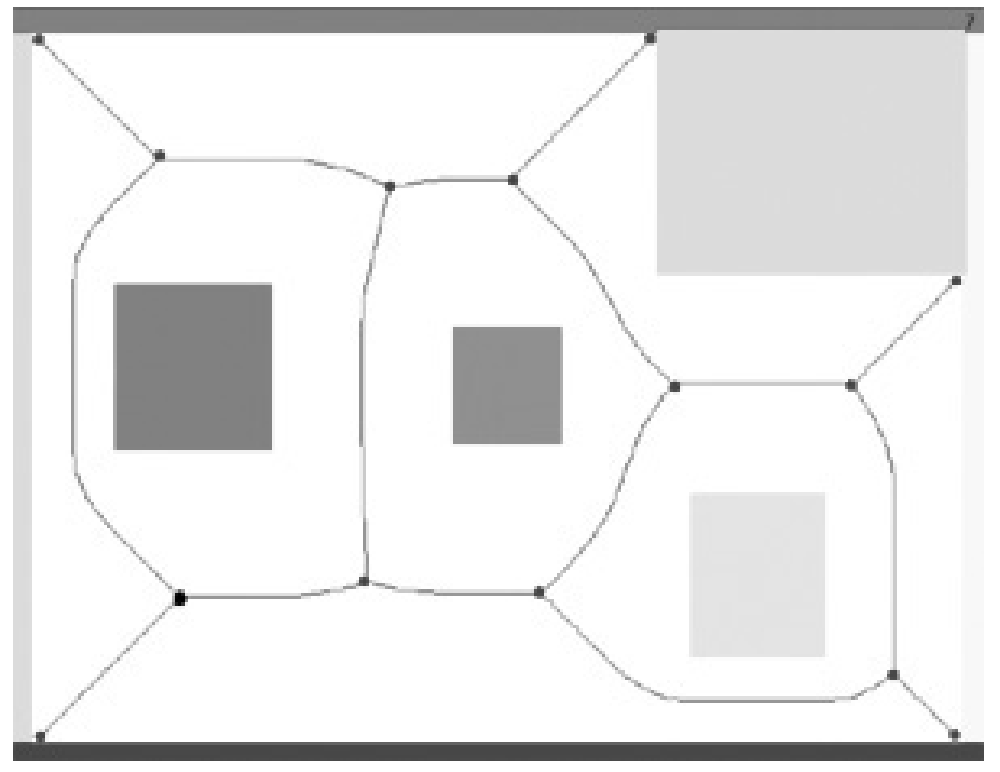
\includegraphics[width=0.5\textwidth]{fig-gvd}
  \caption{An example of good topological map, the rectangles represent the obstacles}
  \label{fig:gvd}
\end{figure}

Some topological map is the abstraction of a \(1\)-dimensional roadmap, which is geometric structures embedded in the free space with three properties: accessibility (it is possible to plan a path between two points onto the roadmap), connectivity (move towards the vicinity of the target point along the roadmap), and departability (reach the target).
To see why the roadmap needs to be only \(1\)-dimensional, consider a point-GVD \(G\) in \(\R^3\), \(G\) consists of \(2\)-dimensional manifolds. The overlap of these \(2\)-dimensional sheets is a \(1\)-dimensional structure called the generalized Voronoi graph (GVG) that the distance from any point in it to adjacent three obstacles are same~\cite{choset1996sensor}. Although the GVG satisfies accessibility and departability, it is not guaranteed to be connected in general. In 1995, Choset and Burdick introduced an extension of GVG called the hierarchical generalized Voronoi graph (HGVG), which is also retract-like. But the later is connected under certain conditions in~\cite{choset1996sensor}. Therefore, it could be used to produce the roadmap for performing a motion planning algorithm. For the detail of how to construct such a HGVG incrementally, see~\cite{choset1995sensor}.

However, generally speaking, the roadmaps mentioned above hardly be good topological maps, and there is no \(1\)-dimensional retract for space of dimensions greater than \(2\). In other words, it is hard to generate good topological maps for \(\R^m\) with \(m>2\).

\subsection{Task Decomposition}
According to the definition of good topological map above, restracts work as good maps because the retraction naturally offers the accessibility, departability, and the retract is connected in every connected components of the free space by the continuity of the retraction function. Moreover, it preserves the cardinality of the first fundamental group as well.

As pointed earlier, we cannot define a \(1\)-dimensional retract of a space with dimension at least \(3\). Nevertheless, a topological map of a \(2\)-dimensional work space can be used to decompose a multi-dimensional configuration space into a set of contractible regions.
Therefore, we can find good maps through retraction in each region and put them back together through the topological adjacency relationship from the original work space. The result is called \emph{piecewise retract} by Choset and Rizzi. Notice that although the piecewise retract may be a bad topological map most times, it consists of smaller good maps for subsets of the configuration space and thus works well for a motion planner.
For examples of applications of piecewise retract, see~\cite{DBLP:conf/isrr/ChosetR03}.
\section{Homotopic Path Similarity in Motion Planning}\label{sec:sim}
%%% Local Variables:
%%% mode: latex
%%% TeX-master: "report"
%%% End:

As mentioned in the introduction, many applications of robotic motion planning benefit from considering multiple homotopically distinct paths rather than a single one. For example when the planning involves multi-agent system or under uncertainty. However, it could be difficult to efficiently check if two paths belong to different homotopy classes. Denny \emph{et al.} proposed metrics to approximate the homotopic similarity between two paths and showed how to compute this approximate similarity efficiently~\cite{denny2018topology}.

\subsection{Probabilistic Path Similarity Metric}
Instead of determine if two paths are in the identical homotopy class, we want to have a metric approximate how likely two paths are in the same homotopy class.
\begin{definition}
  A \emph{path} \(\pi_m=\{q_1,q_2,\dots,q_m\}\) is a contiguous sequence of configurations, two configurations \(q_i,q_{i+1}\) are adjacent if \(\delta(q_i,q_{i+1})\le r\) where \(\delta\) is a distance function and \(r\) is specified in the problem.
\end{definition}\label{def:path}
\begin{definition}
  Let \(\pi_m\) be a path defined above.
  The \(t\)-resolution path \(\tau\) of \(\pi_m\) is a contiguous sequence of configurations discretized at \(t_{\mathrm{res}}\) steps, where \(t_{\mathrm{res}}\) is a resolution for a parametric representation \(t\in[0,1]\) of \(\pi_m\), where \(t=0\) is \(q_1\) and \(t=1\) is \(q_m\). Let \(\tau^k\) denote the \(k_{th}\) configuration of \(\tau\), \(k\in [0,1]\).
\end{definition}
Let \(A\) be the set of all \(t\)-resolution. Let \(\mu:A\times A\to [0,1]\) be a path similarity metric.
If \(\mu\) is of high-quality, then for any two paths \(\alpha, \beta\in A\), \(\mu(\alpha,\beta)=0\) means \(\alpha\) and \(\beta\) are in different homotopy classes where \(\mu(\alpha,\beta)=1\) means their homotopy classes are identical. Moreover, for all \(0<\mu(\alpha,\beta)<1\), the value represents the probability that \(\alpha\) and \(\beta\) are with the same homotopy class.
\subsection{Local Planner Success Similarity}
Denny \emph{et al.} introduced a naive similarity metric based a common subroutine of sampling-based motion planners~\cite{kavraki1996probabilistic}, called the Local Planner Success Similarity (LPSS), see Figure~\ref{fig:lpss}.
\begin{figure}
  \begin{algo}
    \textul{\(\textsc{Local Planner Success Similarity }(\tau_1, \tau_2, \Delta)\):}\+
    \\ \Comment{\(\text{\(\tau_1,\tau_2\) are \(t\)-resolution paths, \(\Delta\) is a local planner.}\)}
    \\ \(s\from 0, n\from 0\)
    \\ for \(t\in[0,1]\) at \(t\)-resolution increments do\+
    \\ if \(\Delta(\tau^t_1,\tau^t_2)\) then\+
    \\ \(s\from s+1\)\-
    \\ \(n\from n+1\)\-
    \\ return \(\frac{s}{n}\)\-
  \end{algo}
  \caption{Algorithm for computing Local Planner Success Similarity}
  \label{fig:lpss}
\end{figure}
The LPSS essentially computes a proportion of successful local planning attempts to total attempts between configurations of the two paths with the same \(t\) value. \(\mu=1\) in this metric guarantee the two paths are in the same homotopy class. The value of \(\mu\) close to \(1\) implies the homeomorphism between two paths are likely to exist. Conversely, If the value of \(\mu\) is near \(0\), they are unlikely in the same class. This algorithm would not yield \(0\) value since the start and goal configurations of \(\tau_1,\tau_2\) are the same. This method is not a good approximation of the similarity metric since it only tries one possible transformation. However, if it correctly determines two paths are in the same class, it has a byproduct that tell us how one can deform into another.
\subsection{Topology-based Edit Distance Similarity}
Based on topological reasoning, Denny \emph{et al.} suggested another similarity metric called Topology-Based Edit Distance Similarity (TBEDS)  that compares the portions of the work space each path accesses.
As shown in Figure~\ref{fig:tbeds}, the algorithm converts each path into a string and uses edit distance as the metric.
\begin{figure}
  \begin{algo}
    \textul{\(\textsc{Topology-based Edit Distance Similarity}(\tau_1, \tau_2, \Delta)\):}\+
    \\ \Comment{\(\text{\(\tau_1,\tau_2\) are \(t\)-resolution paths, \(\Delta\) is a local planner.}\)}
    \\ \(s_1\from\textsc{TOPOLOGYBASEDSTRING(\(\tau_1\))}\)
    \\ \(s_2\from\textsc{TOPOLOGYBASEDSTRING(\(\tau_2\))}\)
    \\ \(d\from\textsc{LEVENSHTEINDISTANCE(\(s_1,s_2\))}\)
    \\ return \(1-\frac{d}{\max{(|s_1|,|s_2|)}}\)\-
  \end{algo}
  \caption{Algorithm for computing Topology-based Edit Distance Similarity}
  \label{fig:tbeds}
\end{figure}
In this algorithm, the method for converting a path into the topology-based string assumes the work space of the robot has been tetrahedralized and converted into a Reeb Graph. For details of this method, see~\cite{denny2018topology}.

If a value of one is returned in this metric, then the paths taken by the point of interest of the robot are in the same homotopy classes of the work space. However, this does not mean the homotopy classes of \(\tau_1,\tau_2\) are same. It still depends on which interest point the algorithm choose and the exact problem. On the other hand, the value close to \(0\) does imply two paths are in different homotopy classes.

Applications of extracting homotopically distinct paths from a roadmap through those metric exist in~\cite{denny2018topology}.
\section{Discussion}\label{sec:dis}
%%% Local Variables:
%%% mode: latex
%%% TeX-master: "report"
%%% End:
In this survey, we reviewed recent progress on several applications of topology in robot motion planning, namely, the topological complexity of the configuration space in motion planning, topological maps for building motion planners or producing concise route, approximate homotopic path similarity in motion planning.
We then went through the basic setting of the problem, introduced configuration spaces of some classic mechanical system, and explored the properties of four topological complexities of the topological space.
There are some open problems regarding the homotopy invariant \(\mathbf{TC}(X)\) such as the rational version of \(\mathbf{TC}(X)\), symmetric motion planning, as well as motion planning in aspherical spaces, see survey~\cite{farber2006topology}.

Choset and Rizzi applied their task decomposition strategy to two classes of practical problems to build ``good'' topological maps. In the future, we can expect more problems can be solved with task decomposition and some more general techniques be designed in order to exploit this tool on motion planning. On the other hand, the practical interest of considering multiple homotopically distinct paths in certain problems motivate us to explore more on finding efficient way to compute a good approximation of the homotopic path similarity and developing algorithms that produce homotopically distinct paths through these metrics.

\paragraph*{Acknowledgment} The authors would like to thank Kyle Fox for instructions into Computational Topology and some helpful discussions.

\bibliography{ref}
\bibliographystyle{plain}
\end{document}